\scanpage{70}
% archive sheet number: 69

\unsure{\deleted{l}g|\deleted{a}g}oing from the category of proper and smooth schemes over $k$ to graded F-crystals, \deleted{compatible} which is additive (for the sum of the $X$ ) and compatible with $\otimes$ \inserted{\handwritten{once tensored with $\unsure{\mathbb{Q}|Q}_p$}}\handwritten{\begin{tikzpicture}[x=1cm,y=1cm,baseline=0cm]\draw[thin] (0,-.45).. controls (-.02,-.1) and (.12,-.06)..(.3,-.06)--(2.3,-.06).. controls (2.38,-.06) and (2.4,0)..(2.4,.17);\end{tikzpicture}} (the $\otimes$ of schemes being the cartesian product) in a way compatible wit\unsure{\deleted{v}h|\deleted{c}h} the associativities and commutativities (both for the sum and for the product), taking care to use the Koko rule for the commutativity constraint. Moreover, modulo verifications which have not yet been made by Berthelot, but which cannot fail to come out soon, the preceding functor is even defined by taking as morphisms algebraic correspondences up to algebraic equivalence\handwritten{\begin{tikzpicture}[x=1cm,y=1cm,baseline=0cm]\draw[gray,thin] (0,.4).. controls (.25,.05) and (.3,-.25)..(.2,-.5);\end{tikzpicture}}, and goes to the \uline{nondegenerate} F-crystals; to be precise, it must be\handwritten{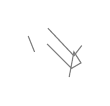
\begin{tikzpicture}[x=1cm,y=1cm,baseline=0cm]\draw[gray,thin] (-.4,.22)--(-.32,.02);\draw[gray,thin] (-.15,.32)--(.18,-.03)--(.28,.1);\draw[gray,thin] (-.16,.12)--(.15,-.19)--(.27,-.12)--(.18,.02)--(.12,-.3);\end{tikzpicture}} true that for every $i$, there exists a $V_i$ :\deleted{in} $H^i\handwritten{\longrightarrow (}H^i\handwritten{)^{\unsure{\deleted{\sigma}\sigma|\sigma}}}$ such that $F\ V_i=p^i\ \mathrm{id}$ , $V_iF=p^i\ \unsure{\deleted{\mathrm{u}}\mathrm{i}|\deleted{\mathrm{i}}\mathrm{u}|\mathrm{i}}\mathrm{d}$ (This is in any case true if $X$ lifts to characteristic 0) Modulo this verification, one thus finds a functor
\[
H^{\handwritten{*}}_{\mathrm{cris}}\substack{\deleted{\unsure{\mathbb{W}}}\\\handwritten{\unsure{\otimes}\mathbb{Q}_p}}:\text{proper smooth schemes over }k\handwritten{\longrightarrow \mathrm{Grad}\unsure{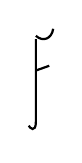
\begin{tikzpicture}[x=1cm,y=1cm,baseline=0cm]\draw[thick] (0,.4)--(0,-.65).. controls (0,-.8) and (-.08,-.73)..(-.09,-.7);\draw[thick] (0,0)--(.17,.06);\draw[thick] (0,.44).. controls (.09,.36) and (.2,.4)..(.22,.53);\end{tikzpicture}}(}\mathrm{F}\unsure{\mathbb{C}|\mathrm{C}|\mathrm{c}|\mathrm{e}}\mathrm{riso}^{\handwritten{+}}(k)\handwritten{)}\ ,
\]
\handwritten{\begin{tikzpicture}[x=1cm,y=1cm,baseline=0cm]\draw[gray,thin] (0,-.35).. controls (.1,-.1) and (.18,.1)..(.16,.4);\end{tikzpicture}}compatible with\deleted{,} everything (a ``cohomolog\unsure{\deleted{ic}y|\deleted{y}ic}\deleted{al} functor'' in the terminology of Kleiman's exposition \handwritten{[\quad]}). Of course, one has $H^{\handwritten{2}}_{\mathrm{cris}}(P^1)=\mathbb{W}(-1)$ , more generally one should have (when Berthelot has \unsure{worked|worked} well
\[
H^{2d\deleted{\unsure{*}}}_{\mathrm{cris}}(X)\handwritten{\simeq}\mathbb{W}(-d)
\]
if $X$ is geometrically connected and of dimension $d$, (canonical isomorphism, compatible with multiplication ...). Assuming the yoga of motives (one needs here the graded structure of the category of motives over $k$, to be able by the Koko rule to fiddle with the natural commutativity constraint on motives, coming from the commutativity isomorphism $X\mathrm{x}Y\handwritten{\simeq}Y\mathrm{x}X$ on schemes ...) one will have a canonical homomorphism of gerbes
\[
\handwritten{\unsure{\Pi|\deleted{\Pi}\Pi}}(k)_{\handwritten{\mathbb{Q}_p}}\handwritten{\longleftarrow}\underline{G}(k)\ ,\qquad
\handwritten{\text{associated with the }\inserted{\text{$\otimes$-functor}}\begin{tikzpicture}[x=1cm,y=1cm,baseline=-.1cm]\draw[thin] (0,-.4).. controls (-.12,.05) and (.05,.3)..(.48,.35)--(1.65,.43).. controls (1.8,.43) and (1.85,.55)..(1.85,.7);\end{tikzpicture}\mathrm{Mot}(k)\longrightarrow\mathrm{Fcriso}(k)}
\]
where $\handwritten{\Pi}(k)$ i\unsure{\deleted{z}s|\deleted{s}s} the gerbe associated with the Tannakian category (over $\underline{Q}$)
